\documentclass[11pt,oneside,letterpaper]{article}

% graphicx package, useful for including eps and pdf graphics
\usepackage{graphicx}
\DeclareGraphicsExtensions{.pdf,.png,.jpg}

% basic packages
\usepackage{color}
\usepackage{parskip}
\usepackage{float}
\usepackage{microtype}
\usepackage{url}

% text layout
\usepackage{geometry}
\geometry{textwidth=16.75cm} % 15.25cm for single-space, 16.25cm for double-space
\geometry{textheight=22.5cm} % 22cm for single-space, 22.5cm for double-space

% helps to keep figures from being orphaned on a page by themselves
\renewcommand{\topfraction}{0.85}
\renewcommand{\textfraction}{0.1}

% bold the 'Figure #' in the caption and separate it with a period
% Captions will be left justified
\usepackage[labelfont=bf,labelsep=period,font=small]{caption}

% review layout with double-spacing
%\usepackage{setspace}
%\doublespacing
%\captionsetup{labelfont=bf,labelsep=period,font=doublespacing}

% cite package, to clean up citations in the main text. Do not remove.
\usepackage{cite}
%\renewcommand\citeleft{(}
%\renewcommand\citeright{)}
%\renewcommand\citeform[1]{\textsl{#1}}

% Remove brackets from numbering in list of References
\renewcommand\refname{\large References}
\makeatletter
\renewcommand{\@biblabel}[1]{\quad#1.}
\makeatother

\usepackage{authblk}
\renewcommand\Authands{ \& }
\renewcommand\Authfont{\normalsize \bf}
\renewcommand\Affilfont{\small \normalfont}
\makeatletter
\renewcommand\AB@affilsepx{, \protect\Affilfont}
\makeatother

%%% TOC
\usepackage{patchcmd}
\makeatletter
\patchcommand\@starttoc{\begin{quote}}{\end{quote}}
\usepackage{tocloft}
\renewcommand{\cftsecleader}{\cftdotfill{\cftdotsep}}

%%% TITLE %%%
\title{\vspace{2cm} \LARGE \bf
Seasonal influenza circulation patterns and projections for 2016-2017
}

\author[1]{Trevor Bedford}
\author[2]{Richard A.\ Neher}

\affil[1]{Vaccine and Infectious Disease Division, Fred Hutchinson Cancer Research Center, Seattle, WA, USA}
\affil[2]{Max Planck Institute for Developmental Biology, T\"ubingen, Germany}

\date{September 16, 2016}

\begin{document}

\maketitle

\tableofcontents

\pagebreak

%%% A/H3N2 %%%
\section*{A/H3N2}
\addcontentsline{toc}{section}{A/H3N2}

\textbf{Despite the late-season 3c3.a epidemic in the USA, we predict clade 3c2.a viruses will continue to predominate in the H3N2 population. Within clade 3c2.a, the 171K variant has spread rapidly so that the majority of recent H3N2 infections are comprised of 171K viruses. Barring the emergence of a new antigenic variant, we believe 171K will continue to predominate.}

We base our primary analysis on a set of viruses collected between Sep 2014 and Aug 2016, comprising approximately 100 viruses per month where available and seeking to equilibrate sample counts geographically where possible (Fig.\ \ref{H3N2_counts}). This equilibration attempts to collect equal samples from Africa, China, Europe, Japan/South Korea, North America, Oceania, South America, South Asia, Southeast Asia and West Asia. In the following analysis we collapse samples from China, South Asia, Southeast Asia, Japan and Korea into a single region referred to here as ``Asia'', resulting in Asia possessing greater sample counts than North America or Europe. The only month that significantly departs from equitable sampling is Aug 2016 with 38 viruses, primarily from Europe and North America. We subsample to 100 viruses per month and not more to keep sample counts as equitable as possible across space and time. Repeating mutation and clade frequency calculations with up to 200 viruses per month and region yields similar results (see below).

\begin{figure}[H]
	\centering
	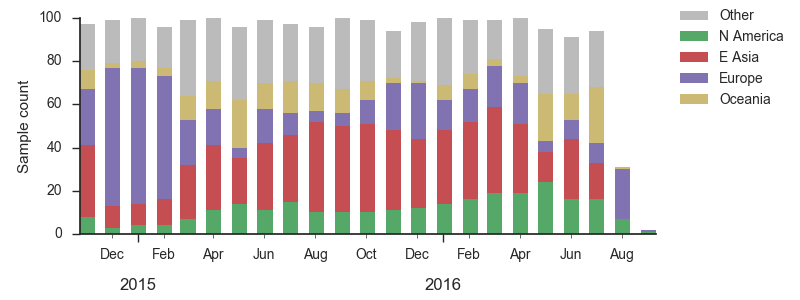
\includegraphics[width=0.95\textwidth]{../figures/sep-2016/H3N2_counts.png}
	\caption{\textbf{Sample counts through time and across regions.}
	This is a stacked bar plot, so that most months there are $\sim$100 total samples and $\sim$15 samples each from North America and from Europe.
	}
	\label{H3N2_counts}
\end{figure}

\pagebreak

Viral clades 3c3.a, 3c3.b and 3c2.a emerged from the Texas/2012 background in early 2014 and rapidly spread through the viral population. Subsequently, we have observed competition among these clades, with 3c2.a viruses being globally dominant beginning in 2015 (Fig.\ \ref{H3N2_clades}). Recently, we have observed the steady decline of 3c3.b viruses. At this point, we estimate that they are either extinct or nearly extinct. 3c3.a viruses were largely replaced by 3c2.a viruses starting in 2015. However, we have observed an anomalous late-season epidemic of 3c3.a viruses within the USA from Jan to Aug 2016. Elsewhere in the world, 3c2.a viruses have remained dominant, particularly in Asia, where we estimate 3c2.a frequencies to be $>$95\% throughout 2016.

\begin{figure}[H]
	\centering
	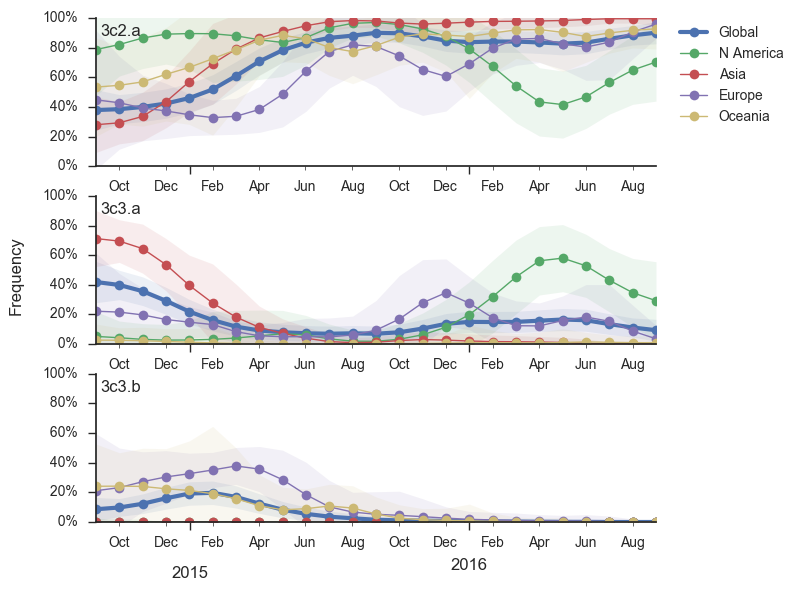
\includegraphics[width=0.95\textwidth]{../figures/sep-2016/H3N2_clades.png}
	\caption{\textbf{Frequency trajectories of H3N2 clades.}
	We estimate frequencies of different clades based on sample counts and collection dates.
	We use a Brownian motion process prior to smooth frequencies from month-to-month.
	Transparent bands show an estimate the 95\% confidence interval based on sample counts.
	The final point represents our frequency estimate for Sep 1 2016.
	}
	\label{H3N2_clades}
\end{figure}

\pagebreak

The late-season 3c3.a epidemic in the USA is puzzling. However, we suspect that this epidemic is due to epidemiologic circumstance rather than the emergence of a selective variant. The strongest evidence for this is that there is not a single clade within 3c3.a that is spreading throughout the USA (Fig.\ \ref{H3N2_3c3a_tree}). Instead, a variety of 3c3.a viruses are spreading, each with different HA1 mutations. The emergence and spread of an adaptive variant would have appeared as a single clade bearing a characteristic epitope mutation. This is not what we see. One small clade, however, carries the S145N and F193S mutations close to the receptor binding site which resulted in antigenic evolution in previous years. The clade is restricted to viruses from US and remains at less than 1\% global frequency. We doubt that these 3c3.a viruses will spread globally. It is conceivable however, that the 2016-2017 USA season could derive from over-summering transmission chains. This would be an unusual event, but not unheard of \cite{bedford2010global}. Still, we believe that 2016-2017 USA season will likely derive from 171K viruses due to their rapid spread (see below).

\begin{figure}[H]
	\centering
	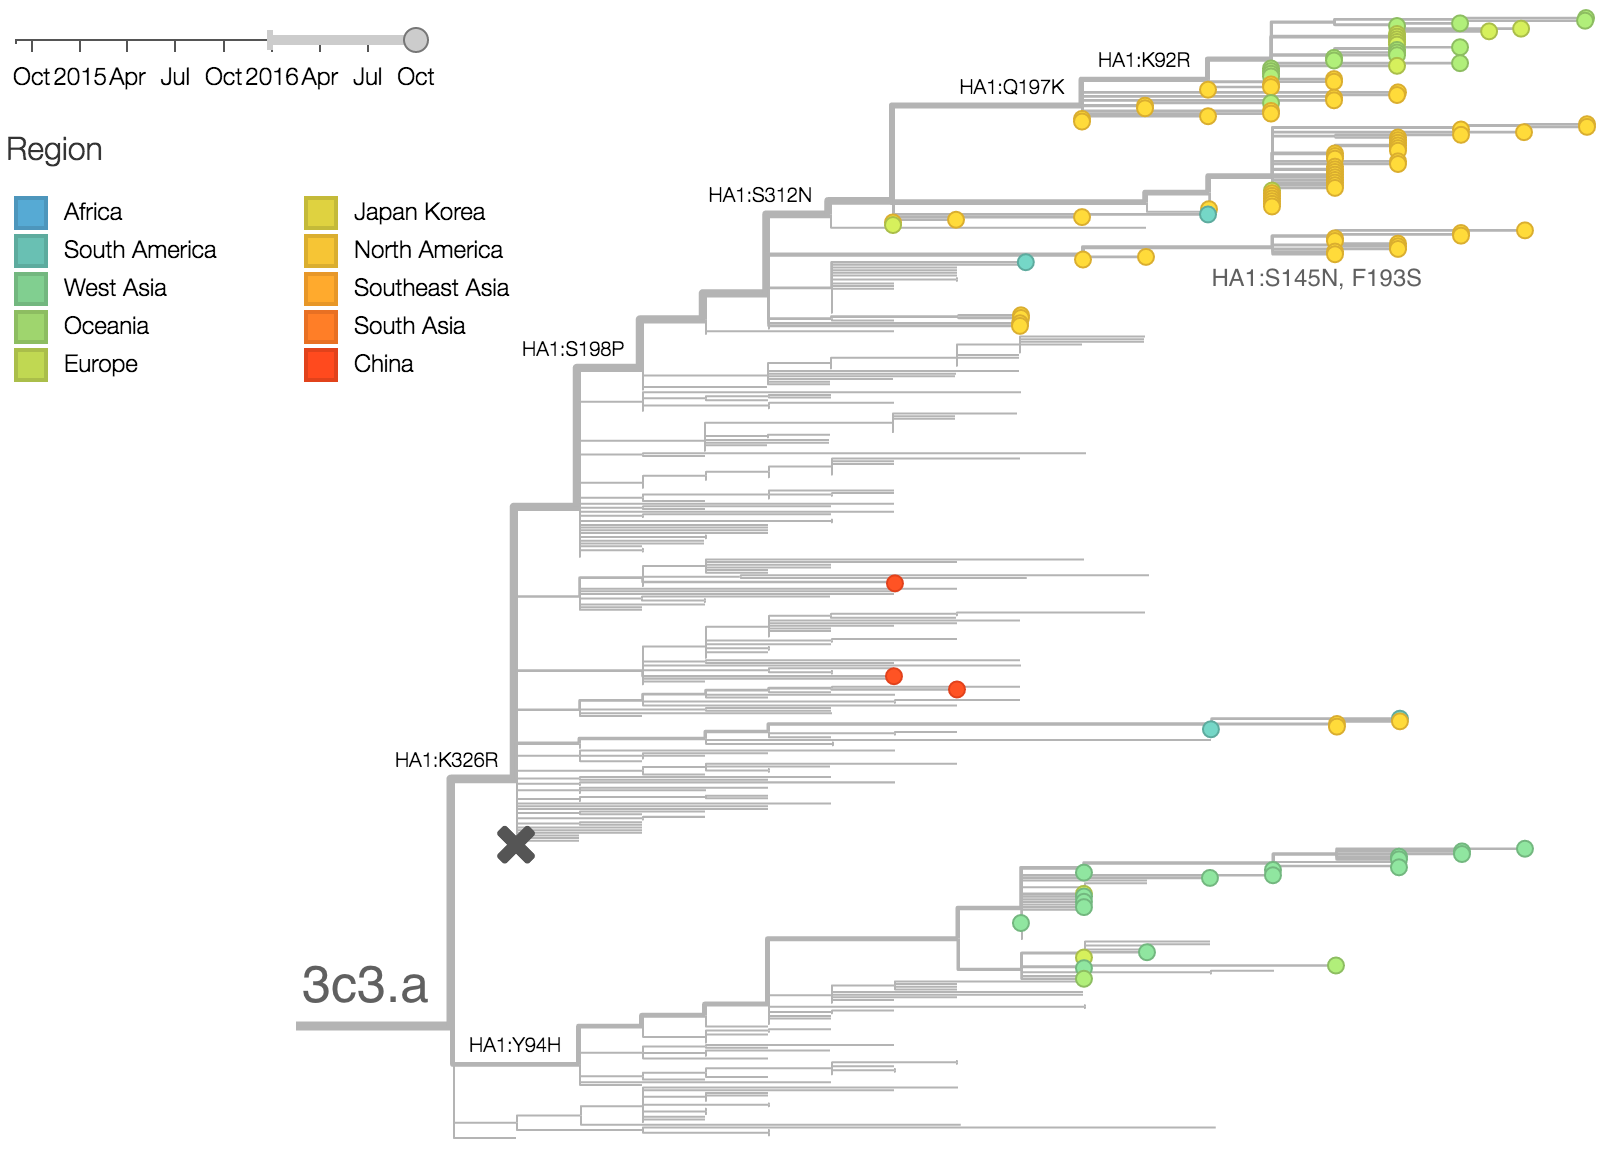
\includegraphics[width=0.9\textwidth]{../figures/sep-2016/H3N2_3c3a_tree.png}
	\caption{\textbf{H3N2 / 3c3.a phylogeny colored by geography.}
	}
	\label{H3N2_3c3a_tree}
\end{figure}

\pagebreak

The dominant 3c2.a viruses have continued to genetically diversify with the emergence of multiple subclades (Fig.\ \ref{H3N2_3c2a_tree}). We observe 3 subclades of decent frequency in 2016 viruses. These are characterized by HA1 mutations 142K/197R, HA1 mutation 197K and HA1 mutation 171K + HA2 mutations 77V/155E. The 171K variant comprises approximately 54\% of 3c2.a viruses collected in 2016.

\begin{figure}[H]
	\centering
	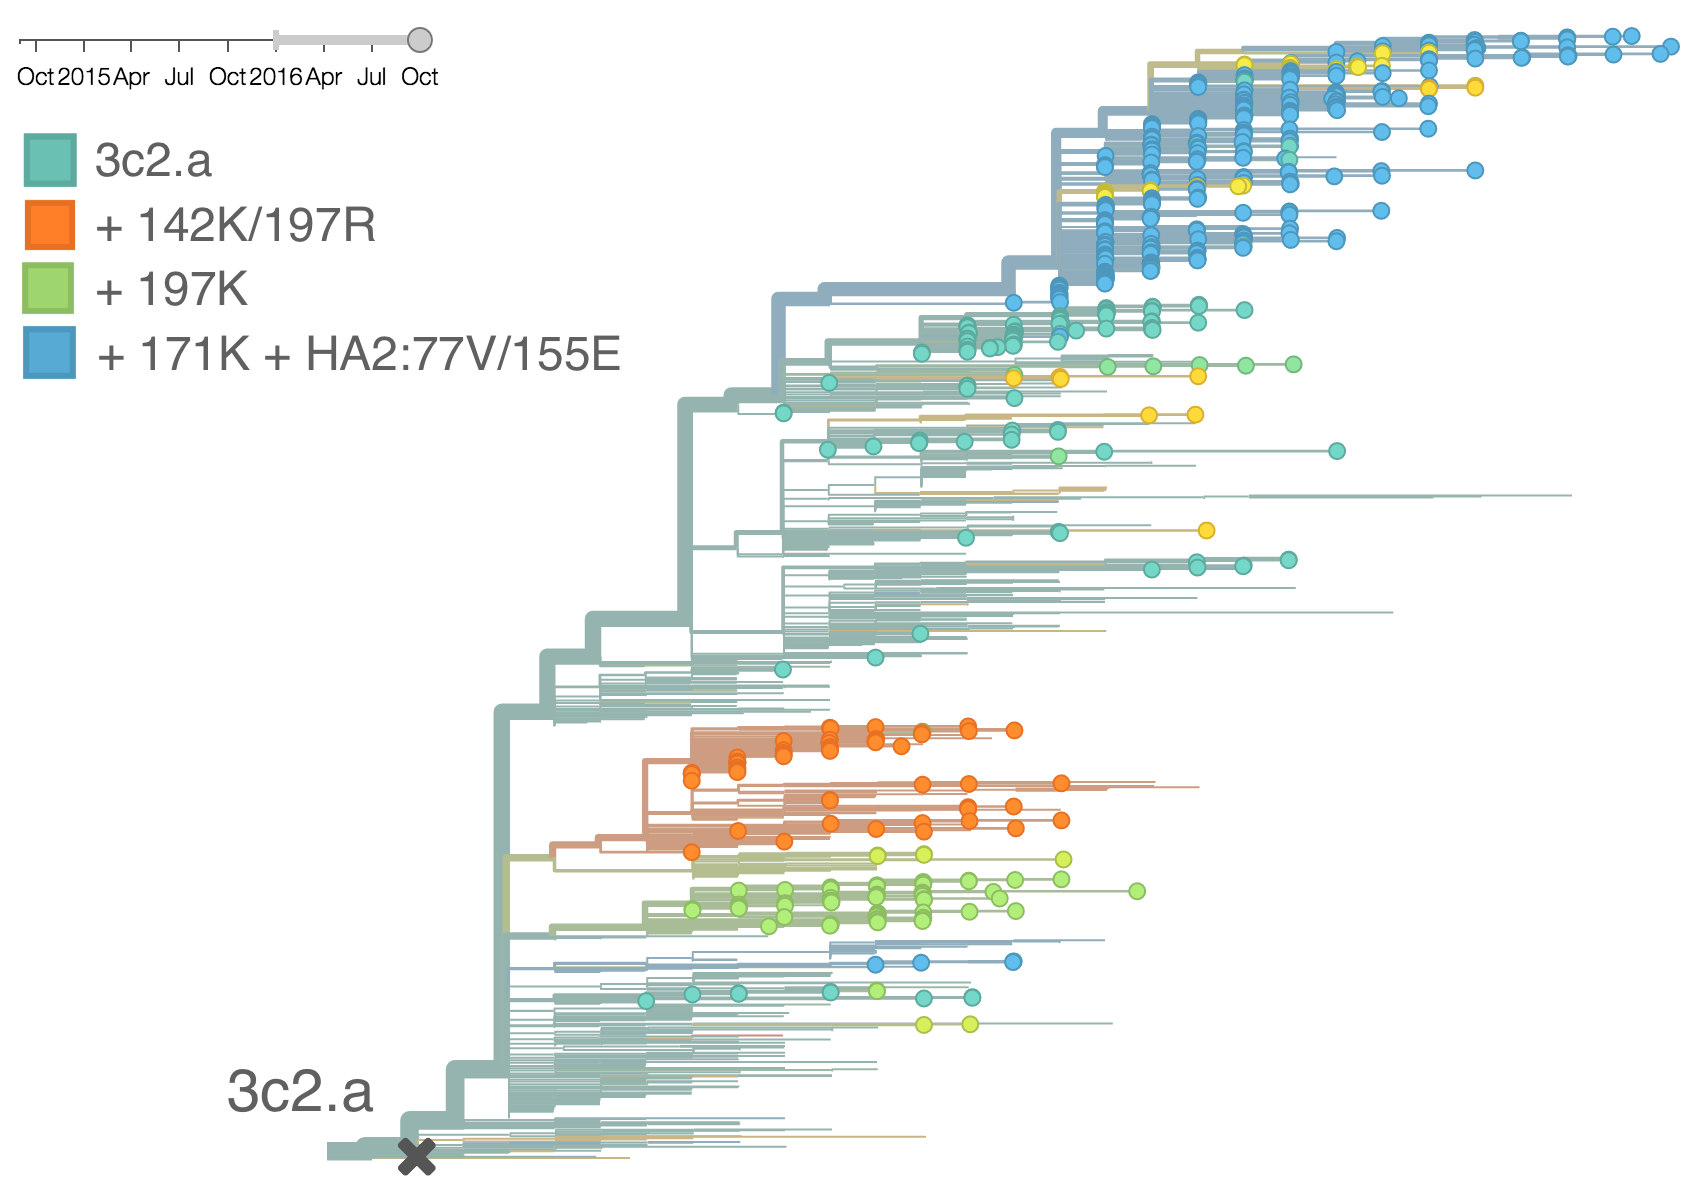
\includegraphics[width=0.9\textwidth]{../figures/sep-2016/H3N2_3c2a_tree.png}
	\caption{\textbf{H3N2 / 3c2.a phylogeny colored by genotype.}
	}
	\label{H3N2_3c2a_tree}
\end{figure}

The 142K/197R clade first emerged around June 2015 and rose to nearly 20\% global frequency in Nov 2015 (Fig.\ \ref{H3N2_mutations}). However, it's declined throughout 2016. We doubt this is a competitive virus. The 197K clade emerged in late 2015 and has slowly grown in frequency since. We estimate that it now comprises $\sim$14\% of H3N2 viruses. However, 197K is at extremely low frequency in Asia with an estimated present-day frequency $\sim$2\%. On the other hand, clade 171K viruses have done remarkably well throughout 2016 and now comprise an estimated 69\% of currently circulating H3N2 viruses. This steady and rapid increase is strongly suggestive of an adaptive origin. Notably, 171K emerged and spread first in Asia, reaching nearly 80\% frequency in April 2016. Higher frequency of 171K in Asia is expected to spread to the rest of the world given historic geographic observations \cite{bedford2015global}.

\pagebreak

\textit{Without strong competition from another novel H3N2 virus, we believe that 171K will continue to increase in frequency in the global population and predominate in the 2016-2017 influenza season.} The continued spread of 171K is fully in line with the predictions we made in Feb 2016 \cite{feb2016report}.

\begin{figure}[H]
	\centering
	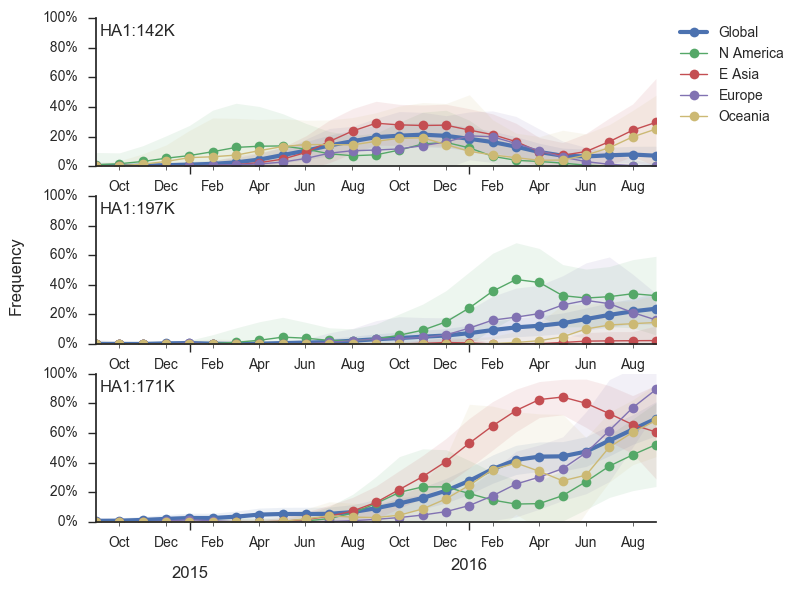
\includegraphics[width=0.95\textwidth]{../figures/sep-2016/H3N2_mutations.png}
	\caption{\textbf{Frequency trajectories of 3c2.a subclades.}
	We estimate frequencies of different clades based on sample counts and collection dates.
	We use a Brownian motion process prior to smooth frequencies from month-to-month.
	Transparent bands show an estimate the 95\% confidence interval based on sample counts.
	The final point represents our frequency estimate for Sep 1 2016.
	}
	\label{H3N2_mutations}
\end{figure}

\pagebreak

Other indicators suggest evolutionary success of 171K viruses. Notably ``local branching index'' \cite{neher2014predicting} supports 171K as a high fitness virus (Fig.\ \ref{H3N2_LBI}). 3c3.a viruses and other clades within 3c2.a and do not show signal in the ``local branching index'' analysis.

\begin{figure}[H]
	\centering
	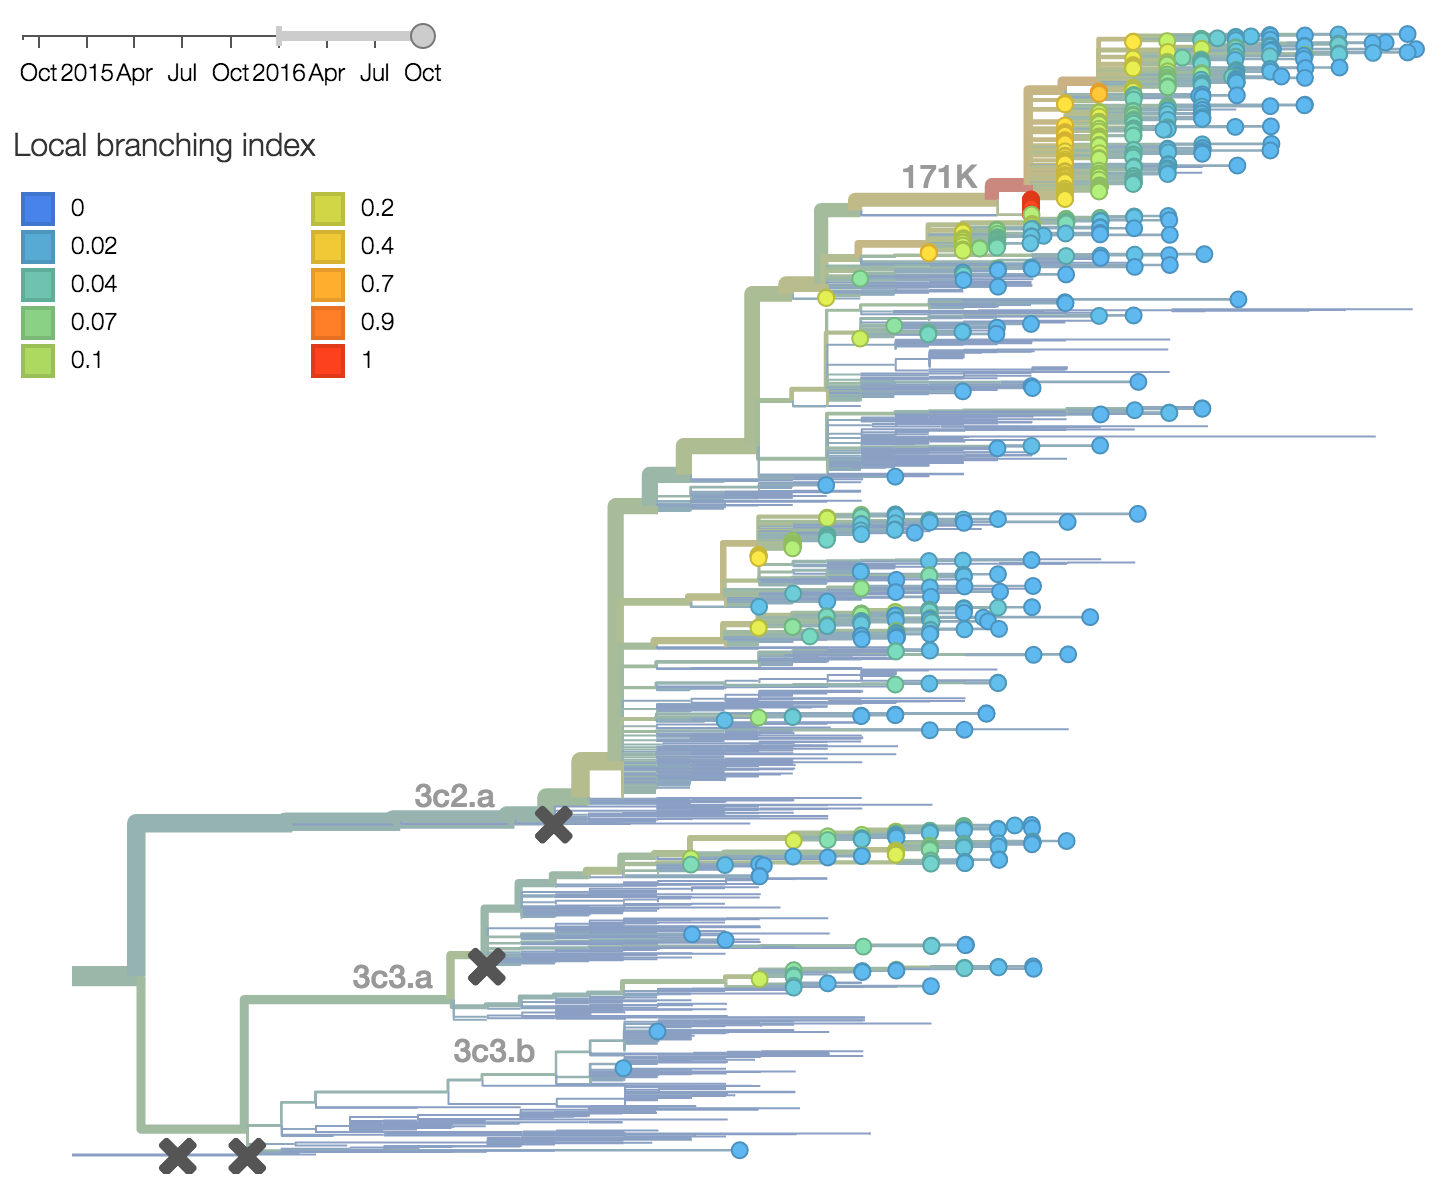
\includegraphics[width=0.9\textwidth]{../figures/sep-2016/H3N2_LBI.png}
	\caption{\textbf{H3N2 phylogeny colored by local branching index.}
	}
	\label{H3N2_LBI}
\end{figure}

Unfortunately, we lack sufficient recent serological data to distinguish antigenic evolution for most subclades within 3c2.a and 3c3.a. These observations derive entirely from genetic data.

\pagebreak

There are a variety of viruses at the base of the 171K clade, possessing HA1:171K along with HA2:77V/155E, but lacking further amino acid changes in HA (Fig.\ \ref{H3N2_171K_basal}).

\begin{figure}[h!]
	\centering
	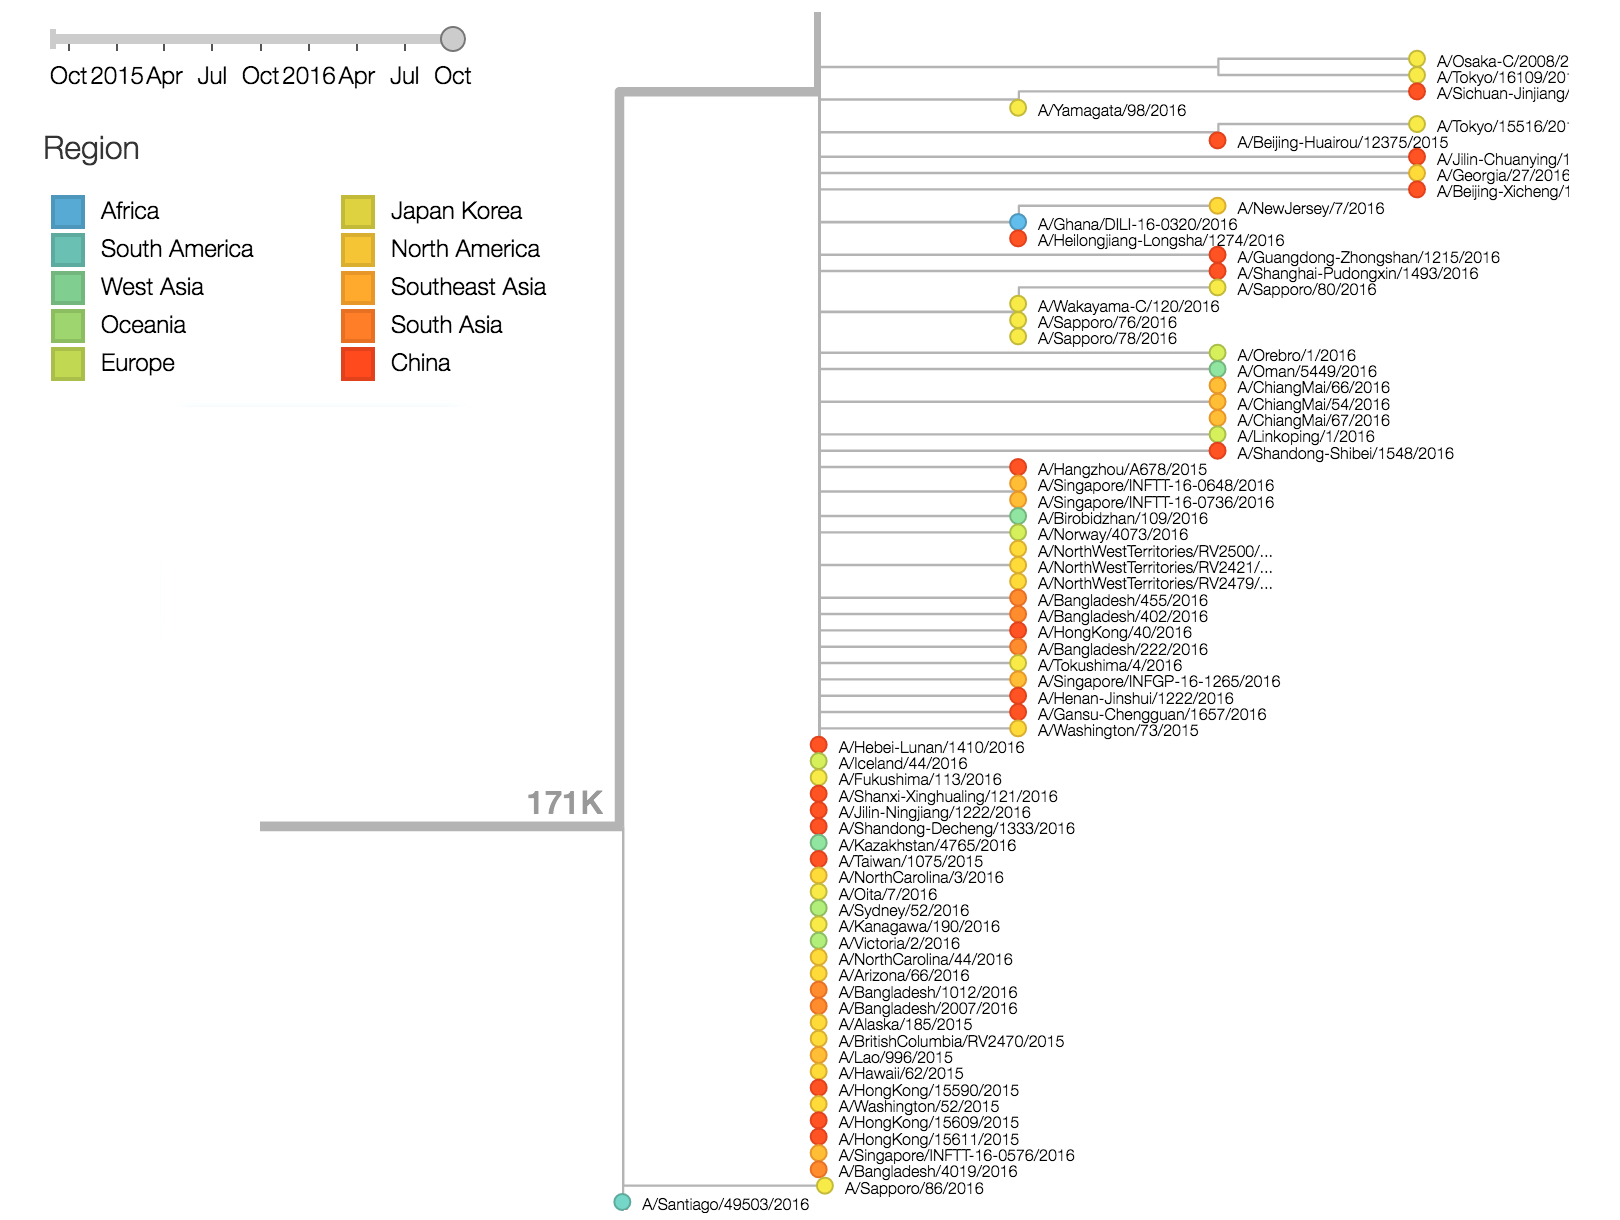
\includegraphics[width=1.0\textwidth]{../figures/sep-2016/H3N2_171K_basal.png}
	\caption{\textbf{Viruses basal to the (HA1:171K, HA2:77V/155E) clade.}
	Viruses are colored according to sampling region.
	}
	\label{H3N2_171K_basal}
\end{figure}

\clearpage
\pagebreak

%%% A/H1N1pdm %%%
\section*{A/H1N1pdm}
\addcontentsline{toc}{section}{A/H1N1pdm}

\textbf{The clade 6b.1, comprising 84N/162N/216T, has continued to rise and predominate in the H1N1pdm population throughout 2016. Almost all circulating H1N1pdm viruses are now 6b.1. There is not yet obvious evolution within this clade.}

As discussed above, we base our primary analysis on a set of viruses collected between Sep 2014 and Aug 2016, comprising approximately 100 viruses per month where available and seeking to equilibrate sample counts geographically where possible (Fig.\ \ref{H1N1pdm_counts}). Recent months through June 2016 have largely sufficient sample counts and sample distributions. There are fewer samples from July to present.

\begin{figure}[H]
	\centering
	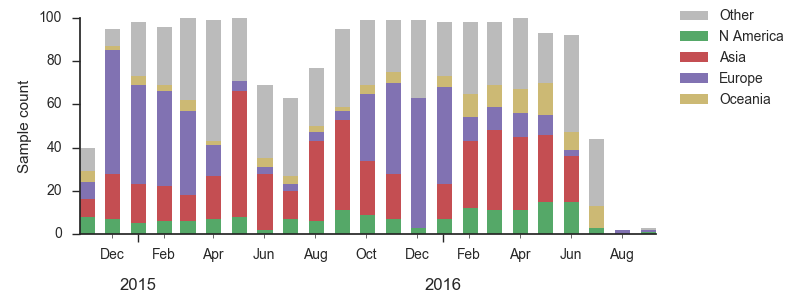
\includegraphics[width=0.95\textwidth]{../figures/sep-2016/H1N1pdm_counts.png}
	\caption{\textbf{Sample counts through time and across regions.}
	This is a stacked bar plot, so that in good months there are $\sim$100 total samples and $\sim$15 samples each from North America and from Europe.
	}
	\label{H1N1pdm_counts}
\end{figure}

\pagebreak

Within clade 6b, two major genetic variants have emerged (Fig.\ \ref{H1N1pdm_tree}). These are clade 6b.1 comprised of HA1:84N/162N/216T and clade 6b.2 comprised of HA1:152T and HA2:174E. Most recent samples have been from 6b.1 viruses, with 85\% of 2016 samples being from 6b.1 viruses.

\begin{figure}[H]
	\centering
	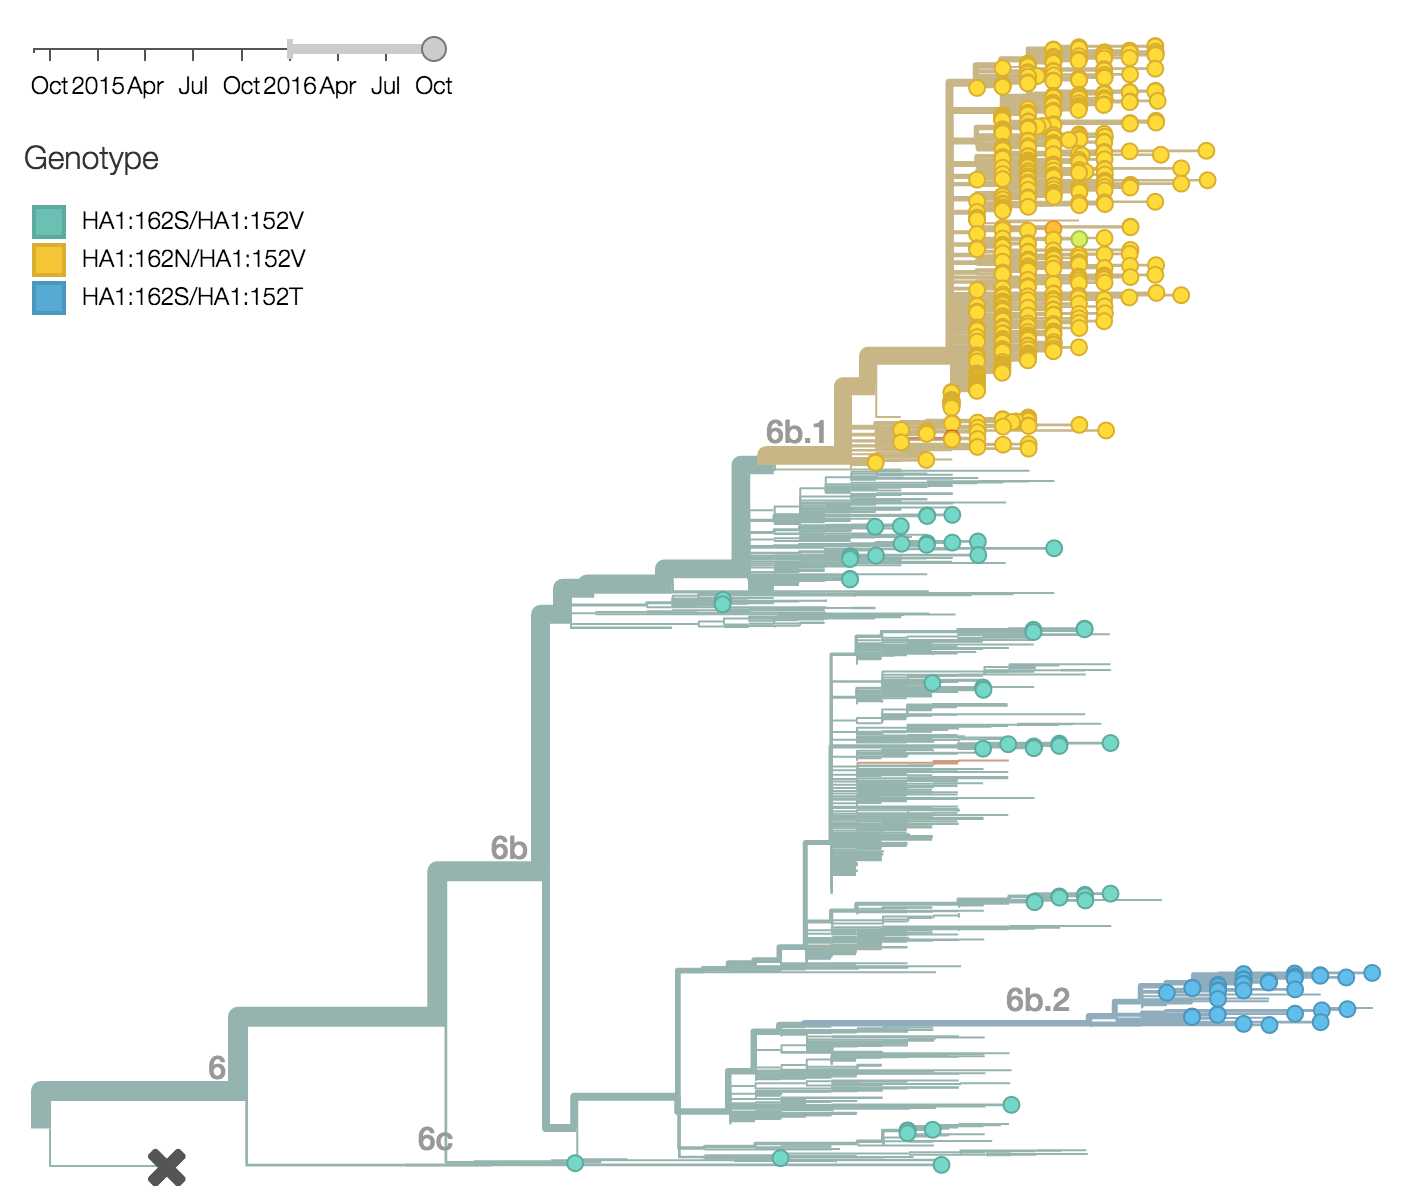
\includegraphics[width=0.9\textwidth]{../figures/sep-2016/H1N1pdm_tree.png}
	\caption{\textbf{H1N1pdm phylogeny colored by genotype.}
	}
	\label{H1N1pdm_tree}
\end{figure}

\pagebreak

At this point, all regions of the world are dominated by 6b.1 viruses (Fig.\ \ref{H1N1pdm_clades}). This clade rose from low frequency in Aug 2015 to reach present day global frequencies of $\sim$98\%. There remain a minority of circulating 6b.2 viruses. We estimate 2\% of H1N1pdm viruses globally to be 6b.2. These are slightly higher prevalence in Asia, but still a distinct minority. We estimate that 6b.1 is at 85\% frequency in Asia, while 6b.2 is at 15\% in Asia. Notably, the frequency of 6b.2 has remained stable for almost 12 months.

\textit{Every indication suggests the continued dominance of 6b.1 viruses, and their extremely rapid rise suggests a selective origin. We are now watching for the emergence of genetic variants within the 6b.1 clade.} Notably, the continued rise and dominance of 6b.1 viruses fits with our predictions from Feb 2016 \cite{feb2016report}.

\begin{figure}[H]
	\centering
	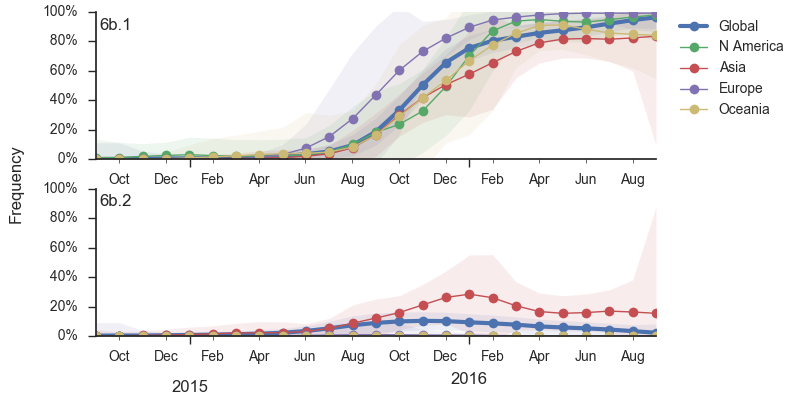
\includegraphics[width=0.95\textwidth]{../figures/sep-2016/H1N1pdm_clades.png}
	\caption{\textbf{Frequency trajectories of H1N1pdm clades.}
	We estimate frequencies of different clades based on sample counts and collection dates.
	We use a Brownian motion process prior to smooth frequencies from month-to-month.
	Transparent bands show an estimate the 95\% confidence interval based on sample counts.
	The final point represents our frequency estimate for Sep 1 2016.
	}
	\label{H1N1pdm_clades}
\end{figure}

\clearpage
\pagebreak

%%% B/Victoria %%%
\section*{B/Vic}
\addcontentsline{toc}{section}{B/Vic}

\textbf{Within clade 1A viruses, the clade 129D/146I/117V has risen to high frequency, but at a rate that suggests a smaller effect of natural selection. At this point, 117V viruses are dominant in the global viral population.}

As above, we base our primary analysis on a set of viruses collected between Sep 2014 and Aug 2016, comprising approximately 100 viruses per month where available and seeking to equilibrate sample counts geographically where possible (Fig.\ \ref{Vic_counts}).

\begin{figure}[H]
	\centering
	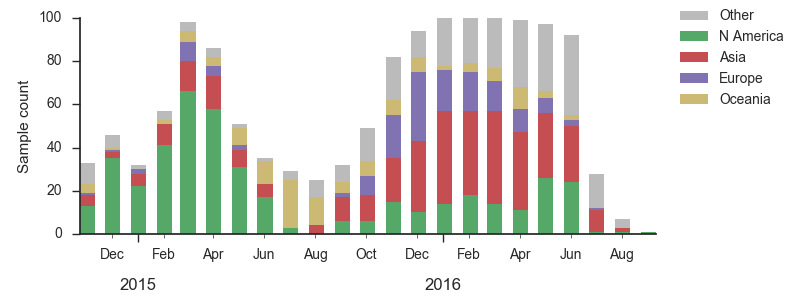
\includegraphics[width=0.95\textwidth]{../figures/sep-2016/Vic_counts.png}
	\caption{\textbf{Sample counts through time and across regions.}
	This is a stacked bar plot, so that in good months there are $\sim$100 total samples and $\sim$15 samples each from North America and from Europe.
	}
	\label{Vic_counts}
\end{figure}

\pagebreak

In the past year, B/Vic clade 129D/146I/117V has dominated the viral population, with 94\% of samples possessing the 117V mutation (Fig.\ \ref{Vic_mutations}). This dominance has increased throughout 2016 and we estimate that currently circulating Vic viruses are 94\% 117V. At this point, we haven't observed new variants of appreciable frequency within the 117V clade and there aren't decent competitors outside the 117V clade.

\begin{figure}[H]
	\centering
	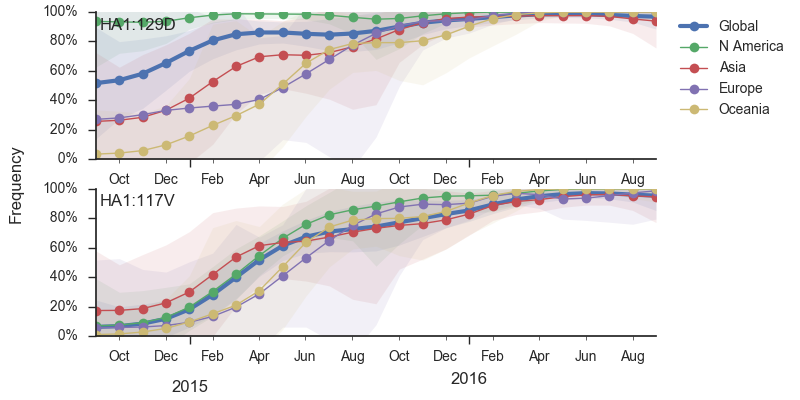
\includegraphics[width=0.95\textwidth]{../figures/sep-2016/Vic_mutations.png}
	\caption{\textbf{Frequency trajectories of B/Vic variants.}
	We estimate frequencies of different clades based on sample counts and collection dates.
	We use a Brownian motion process prior to smooth frequencies from month-to-month.
	Transparent bands show an estimate the 95\% confidence interval based on sample counts.
	The final point represents our frequency estimate for Sep 1 2016.
	}
	\label{Vic_mutations}
\end{figure}

\pagebreak

Additionally, the 117V clade has been growing most quickly and is picked by the local branching index \cite{neher2014predicting} as the currently most successful clade (Fig.\ \ref{Vic_LBI}). \textit{All indicators suggest the continued success of 117V in the coming year.}

\begin{figure}[H]
	\centering
	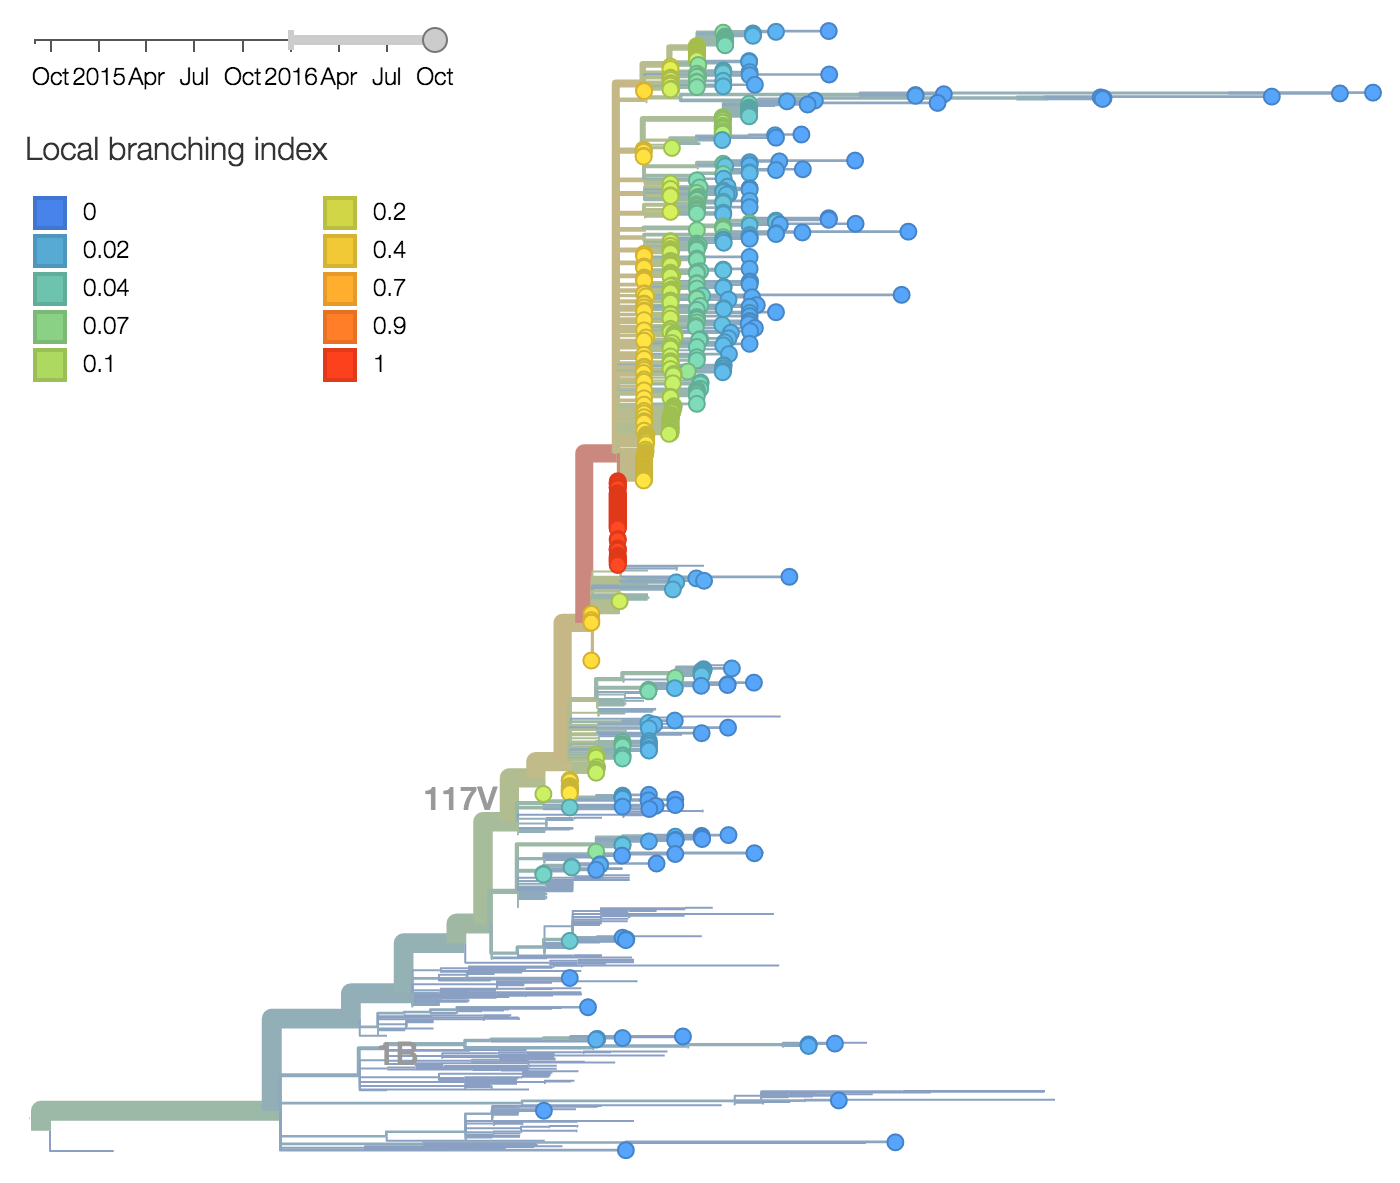
\includegraphics[width=0.9\textwidth]{../figures/sep-2016/Vic_LBI.png}
	\caption{\textbf{B/Vic phylogeny colored by local branching index.}
	}
	\label{Vic_LBI}
\end{figure}

\clearpage
\pagebreak

%%% B/Yamagata %%%
\section*{B/Yam}
\addcontentsline{toc}{section}{B/Yam}

\textbf{Clade 3 has continued to predominate the B/Yamagata population. Within clade 3 the 172Q/251Q subclade has risen to predominate. There is limited diversity within 172Q/251Q viruses, with the largest subclade comprised of 211R viruses.}

As above, we base our primary analysis on a set of viruses collected between Sep 2014 and Jul 2016, comprising approximately 100 viruses per month where available and seeking to equilibrate sample counts geographically where possible (Fig.\ \ref{Yam_counts}).

\begin{figure}[H]
	\centering
	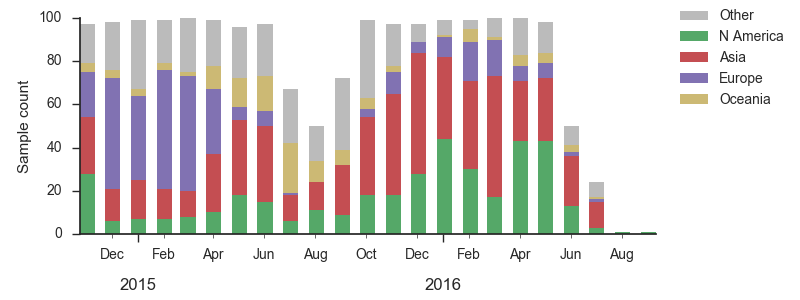
\includegraphics[width=0.95\textwidth]{../figures/sep-2016/Yam_counts.png}
	\caption{\textbf{Sample counts through time and across regions.}
	This is a stacked bar plot, so that in good months there are $\sim$100 total samples and $\sim$15 samples each from North America and from Europe.
	}
	\label{Yam_counts}
\end{figure}

\pagebreak

During 2016, the vast majority of B/Yamagata isolates were of clade 3 viruses (Fig.\ \ref{Yam_clades}). We estimate that the current frequency of clade 2 is now $\sim$2\%. At this rate, we expect clade 2 to go extinct in the coming year.

\begin{figure}[H]
	\centering
	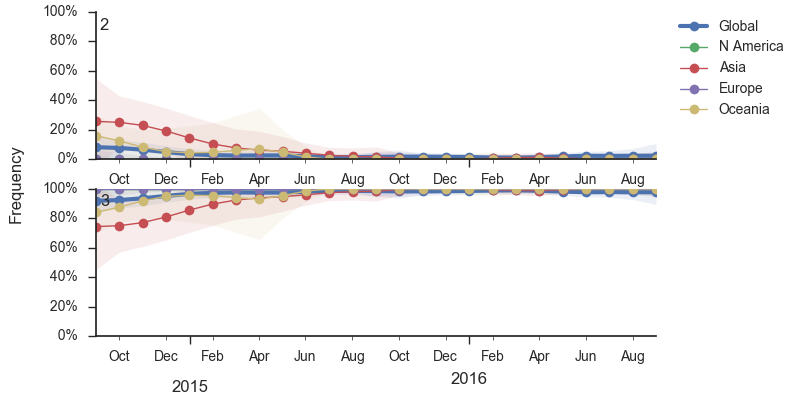
\includegraphics[width=0.95\textwidth]{../figures/sep-2016/Yam_clades.png}
	\caption{\textbf{Frequency trajectories of B/Yam clades.}
	We estimate frequencies of different clades based on sample counts and collection dates.
	We use a Brownian motion process prior to smooth frequencies from month-to-month.
	Transparent bands show an estimate the 95\% confidence interval based on sample counts.
	The final point represents our frequency estimate for Sep 1 2016.
	}
	\label{Yam_clades}
\end{figure}

\pagebreak

Within clade 3, HA1:172Q has predominated throughout 2015 and 2016 (Fig.\ \ref{Yam_tree}). On this background the HA1:251V variant has emerged and on top of 251V, the HA1:211R variant has appeared.

\begin{figure}[H]
	\centering
	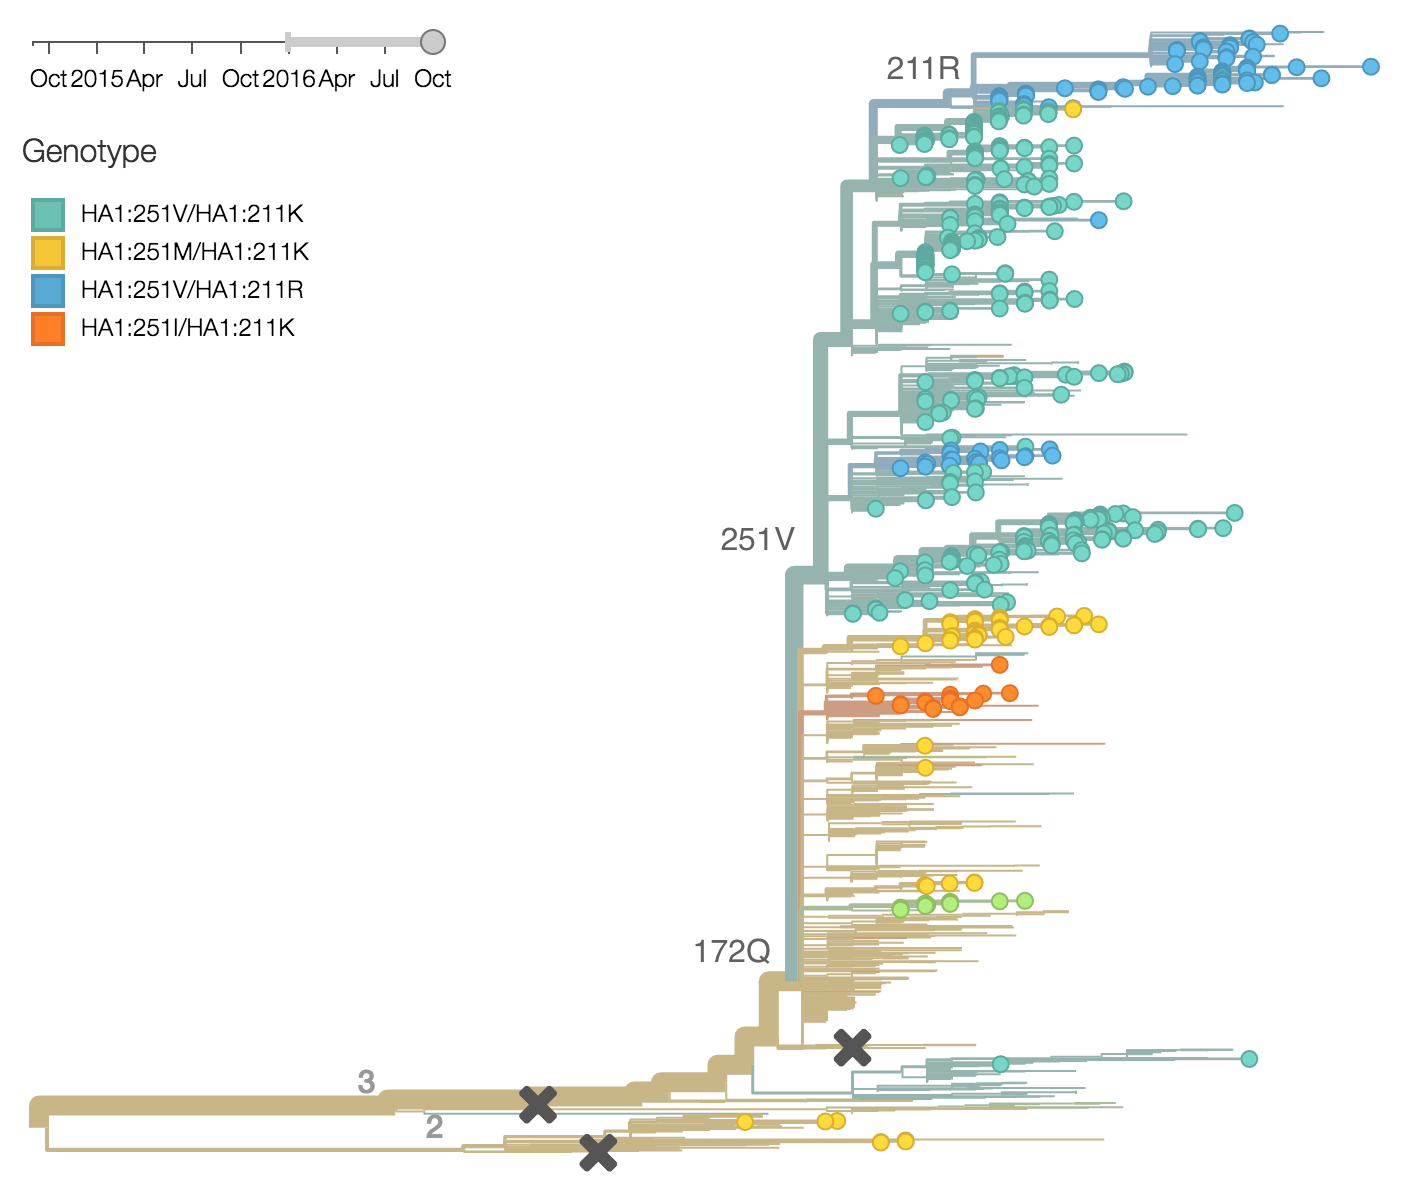
\includegraphics[width=0.9\textwidth]{../figures/sep-2016/Yam_tree.png}
	\caption{\textbf{B/Yam phylogeny colored by genotype.}
	}
	\label{Yam_tree}
\end{figure}

\pagebreak

The 251V clade increased from low frequency in Oct 2014 to predominate in the population (Fig.\ \ref{Yam_mutations}). We estimate that 251V is currently at 79\% globally. The 211R variant rose from low frequency in Apr 2015 to reach 34\% in currently circulating viruses. The rate of increase, however, has been rather mild.

\begin{figure}[H]
	\centering
	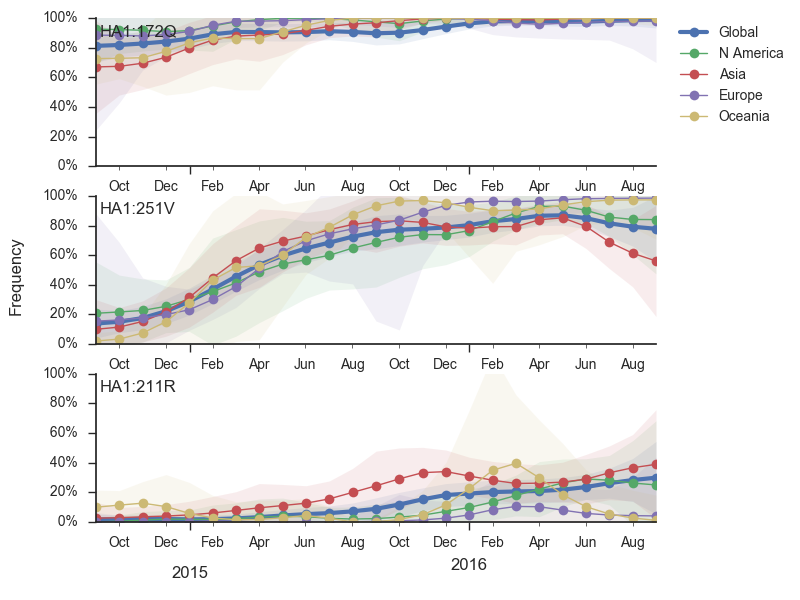
\includegraphics[width=0.95\textwidth]{../figures/sep-2016/Yam_mutations.png}
	\caption{\textbf{Frequency trajectories of B/Yam variants.}
	We estimate frequencies of different clades based on sample counts and collection dates.
	We use a Brownian motion process prior to smooth frequencies from month-to-month.
	Transparent bands show an estimate the 95\% confidence interval based on sample counts.
	The final point represents our frequency estimate for Sep 1 2016.
	}
	\label{Yam_mutations}
\end{figure}

\clearpage
\pagebreak

%%% A/H3N2 (all sequences) %%%
\section*{A/H3N2 (all sequences)}
\addcontentsline{toc}{section}{A/H3N2 (all sequences)}

The clade and mutation frequencies discussed above were based on a limited sequence subsample with an equitable geographical distribution. More accurate region specific trajectories can be estimated using all sequence data available in GISAID. We repeated the clade and mutation frequency estimation using up to 200 sequences per month and region (Fig.\ \ref{H3N2_counts_all}).

\begin{figure}[H]
	\centering
	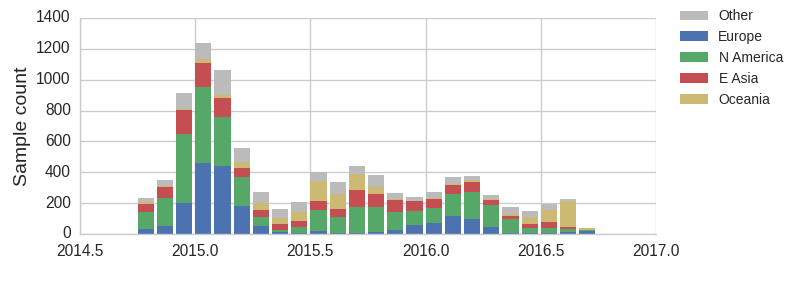
\includegraphics[width=0.95\textwidth]{../figures/sep-2016/H3N2_counts_all.png}
	\caption{\textbf{Sample counts through time and across regions.}
	This is a stacked bar plot, so that in the peak of the 2014-2015 season there are $\sim$700 total samples per month.
	}
	\label{H3N2_counts_all}
\end{figure}

\pagebreak

With this more inclusive sampling, northern hemisphere winter months tend to be dominated by North America and Europe, while other months are dominated by samples from North America, Asia, and Oceania (Fig.\ \ref{H3N2_clades_all}). The global average will track the regions contributing the majority of the sequence data.

\begin{figure}[H]
	\centering
	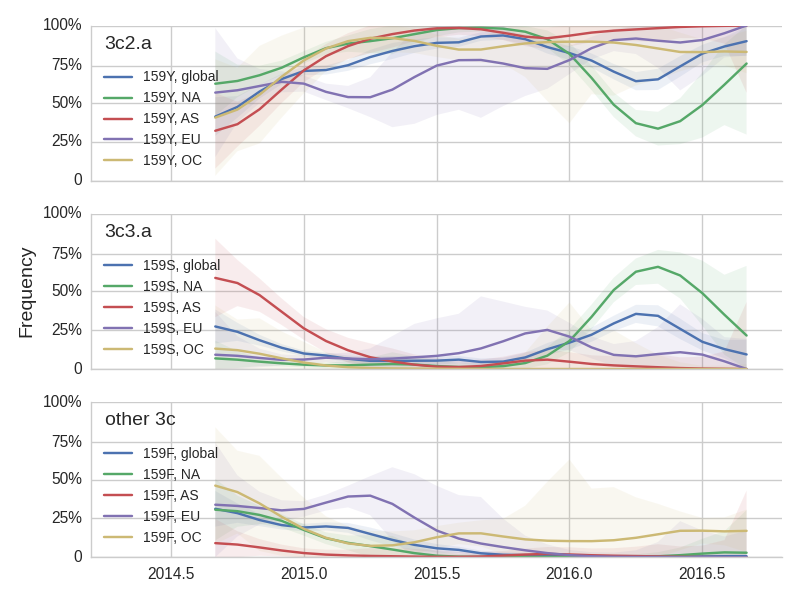
\includegraphics[width=0.95\textwidth]{../figures/sep-2016/H3N2_clades_all.png}
	\caption{\textbf{Frequency trajectories of H3N2 clades.}
	We estimate frequencies of different clades based on sample counts and collection dates.
	We use a Brownian motion process prior to smooth frequencies from month-to-month.
	Transparent bands show an estimate the 95\% confidence interval based on sample counts.
	The final point represents our frequency estimate for Sep 1 2016.
	}
	\label{H3N2_clades_all}
\end{figure}

\pagebreak

The H3N2 clades 3c3.a (159S) and 3c2.a (159Y) show broadly similar trajectories as discussed above (Fig.\ \ref{H3N2_mutations_all}). 3c2.a came to dominate Asia completely, while viruses outside of 3c3.a and 3c2.a continue to circulate at low levels in Oceania. Within 3c2.a, the mutation 171K dominates across all regions.

\begin{figure}[H]
	\centering
	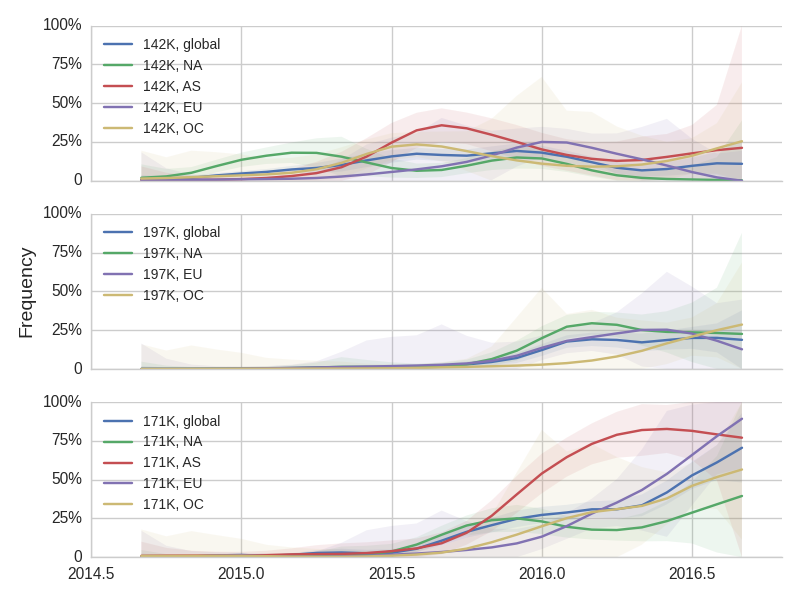
\includegraphics[width=0.95\textwidth]{../figures/sep-2016/H3N2_mutations_all.png}
	\caption{\textbf{Frequency trajectories of H3N2 mutations.}
	We estimate frequencies of different clades based on sample counts and collection dates.
	We use a Brownian motion process prior to smooth frequencies from month-to-month.
	Transparent bands show an estimate the 95\% confidence interval based on sample counts.
	The final point represents our frequency estimate for Sep 1 2016.
	}
	\label{H3N2_mutations_all}
\end{figure}

%%% References %%%
\bibliographystyle{plos}
\bibliography{references}

\end{document}
